% !TEX encoding = UTF-8
% !TEX TS-program = pdflatex
% !TEX root = ../arsclassica.tex
% !TEX spellcheck = it-IT

%************************************************
\chapter{Guide all'uso}
\label{cap:guide}
%************************************************
Lo scopo di questa appendice è formulare delle guide all'utilizzo del software sviluppato a sostengo del lavoro di tesi.

Questa appendice è quindi suddivisa in due sezioni tematiche, una relativa all'utilizzo delle funzionalità offerte dal \pacchettor{} e una relativa all'utilizzo di \acsfont{Sensors} \acs{DLL} per la generazione di dataset da modelli \acs{TSIS}.

\section{Utilizzo del pacchetto RCTBN}\label{sec:package-howto}
Nelle seguenti sottosezioni si illustrano le funzionalità principali offerte da \rctbn{}. Lo scopo è quello di guidare l'utente all'utilizzo del framework delle \acs{CTBN} tramite il succitato pacchetto \lstinline[]|R|.

Prima di addentrarci nella guida all'utilizzo del \pacchettor{} è necessario verificare che il sistema disponga dell'adeguato ambiente \lstinline[]|R| (versione $\ge 3.0$). Inoltre è necessario che il pacchetto \lstinline[]|devtools|\footnote{Il pacchetto \lstinline[]|devtools| è un insieme di funzioni e strumenti finalizzati all'espletamento di processi comuni e fondamentali per lo sviluppo in \lstinline[]|R|. Il codice sorgente di tale pacchetto è disponibile all'indirizzo: \url{https://github.com/hadley/devtools}.} sia correttamente installato. In caso contrario, purché si disponga di una connessione a Internet, è possibile installare l'ultima versione stabile digitando il seguente comando in una nuova sessione \lstinline[]|R|.

\vspace*{8pt}\inputsourcecode[caption={[Installazione del pacchetto \lstinline$devtools$]Installazione del pacchetto \lstinline$devtools$.},language=rstats,numbers=none]{codes/devtoolsinstallation}

A questo punto è possibile procedere all'installazione del \pacchettor{}. Poiché esso non è ancora stato pubblicato nell'archivio online dei pacchetti \lstinline$R$\footnote{Una delle modalità di installazione di pacchetti \lstinline$R$ è tramite connessione a un archivio online in cui essi vengono memorizzati. Tale archivio, chiamato \acf{CRAN}, è raggiungibile al seguente indirizzo: \url{http://cran.r-project.org}.}, la procedura di installazione differisce da quella precedentemente mostrata. A tale scopo si utilizza quindi il pacchetto \lstinline$devtools$ per installare \rctbn{}. Si osservi che il pacchetto \lstinline$devtools$ permette di creare e installare un pacchetto \lstinline$R$ a partire dal suo sorgente (purché esso rispetti le dovute convenzioni e contenga codice eseguibile senza errori), che sia esso online o sul sistema dell'utente, o da un archivio compresso. Perciò, disponendo del sorgente di \rctbn{}, è possibile installarlo come pacchetto \lstinline$R$ digitando le seguenti istruzioni.

\vspace*{8pt}\inputsourcecode[caption={[Installazione del \pacchettor{}]Installazione del \pacchettor{}.},language=rstats]{codes/rctbninstallation}

Si osservi che l'opzione \lstinline$dependencies$ fa sì che tutte i pacchetti da cui \rctbn{} dipende vengano scaricati e installati dall'archivio \acs{CRAN}: anche in questo caso è quindi necessaria una connessione a Internet.

\`E ora possibile utilizzare il \pacchettor{} per l'esecuzione dei vari processi relativi al framework delle \acs{CTBN}. Si osservi che esso viene installato con il nome \lstinline$ctbn$ nella libreria \lstinline$R$.

Tutti gli esempi d'utilizzo che vengono mostrati in questa sezione assumono che la cartella di lavoro sia \lstinline[language=rstats]{"~/Workspace/R/test/ctbn"}. Perciò, come mostrato in seguito, si utilizza il comando \lstinline$setwd$ per impostare la cartella di lavoro.

\subsection{Gestione dei dataset}
Come detto nella \autoref{subsec:rctbn-ds-management} \vpageref{subsec:rctbn-ds-management}, il \pacchettor{} implementa una serie di funzionalità, non correlate concettualmente al framework delle \acs{CTBN}, utili allo svolgimento di operazioni di gestione dei dataset. Lo scopo principale di questo insieme di funzionalità è permettere il caricamento e la compressione su disco dei dataset per le \acs{CTBN}, così da evitare all'utente la ripetizione di tale operazione ogni qual volta egli necessiti di un dataset precedentemente già importato.

Perciò, di seguito si illustra come importare il \ds{2} (descritto nella \vref{sec:dataset-2}).

\vspace*{8pt}\inputsourcecode[caption={[Importazione e serializzazione del \ds{2}]Importazione e serializzazione del \ds{2}.},language=rstats,label=lst:rctbn-import-ds]{codes/importctbnds}
Si osservi che, come anticipato, è indispensabile impostare la corrente cartella di lavoro (comando \lstinline$setwd$) poiché il \pacchettor{} utilizza tale informazione per cercare il dataset da importare. Nello specifico, \rctbn{} cercherà nella cartella di lavoro una cartella \lstinline$dataset$ e dentro questa cercherà una cartella con il nome del primo parametro attuale della funzione \lstinline[language=rstats]{read_dataset}. \`E possibile modificare la cartella in cui \rctbn{} cerca i dataset modificando l'opzione \lstinline$ctbn.data.dir$, impostata di default al valore \lstinline$dataset$, tramite il comando \lstinline[language=rstats]{options}.

La funzione \lstinline[language=rstats]{read_dataset} effettua varie operazioni, che vengono descritte di seguito.
\begin{itemize}
	\item Legge ogni file \acs{CSV} presente nella cartella:\par
	\lstinline[language=rstats]{"~/Workspace/R/test/ctbn/dataset/monza100o"}.\par
	\`E possibile importare file con altre estensioni semplicemente modificando il valore dell'opzione \lstinline$ctbn.data.ext$, impostato all'avvio al valore \lstinline[language=rstats]{"csv"}.
	\item Controlla che ogni struttura tabulare letta contenga la colonna relativa al tempo. Tale informazione è specificabile tramite l'opzione \lstinline$ctbn.col.time$, impostata di default al valore \lstinline[language=rstats]{"time"}.
	\item Controlla che ogni struttura tabulare letta contenga la colonna relativa alla classe. Tale informazione è specificabile tramite l'opzione \lstinline$ctbn.col.class$, impostata all'avvio a \lstinline[language=rstats]{"class"}. Nel caso in cui non si sia interessati ad eseguire tale controllo è possibile ometterlo semplicemente modificando la chiamata in questione come mostrato di seguito:\par
	\lstinline[language=rstats]{read_dataset("monza100o", classcheck = FALSE)}.
	\item Controlla che ogni file contenga altre colonne oltre a quelle relative al tempo e, opzionalmente, alla classe.
	\item Ordina le strutture tabulari importati in base alle rispettive colonne temporali.
	\item Crea un oggetto \lstinline$R$ simile a una tabella hash dove ogni chiave è rappresentata da una stringa, il nome del file importato (senza estensione), e ogni elemento è una tabella (nello specifico un oggetto della classe \lstinline$data.table$) contenente la struttura tabulare importata.
	\item Serializza in modo compresso tale oggetto su file salvando un file \acsfont{RDATA}\footnote{I file con estensione \acsfont{RDATA}, o \acsfont{RDA}, sono dei formati binari che \lstinline$R$ utilizza per la memorizzazione su disco di oggetti appartenenti al suo linguaggio.} nella cartella adibita alla memorizzazione dei dataset importati (specificata dall'opzione \lstinline$ctbn.store.dir$, il cui valore di default è \lstinline[language=rstats]{"data"}). \`E possibile, ma non consigliato, disattivare la serializzazione del dataset importato modificando la chiamata in questione come mostrato:\par
	\lstinline[language=rstats]{read_dataset("monza100o", autosave = FALSE)}.
\end{itemize}

L'output del sorgente \ref{lst:rctbn-import-ds} corrisponde all'oggetto \lstinline$R$ contenente il dataset nelle modalità descritte. Ciò significa che assegnando tale funzione a una variabile sarà possibile operare con il dataset in questione. Ad esempio:

\lstinline[language=rstats]{monzads = read_dataset("monza100o")}.

Si osservi che, nel caso in cui non l'opzione \lstinline$ctbn.verbose$ (posta di default a \lstinline[language=rstats]{TRUE}) non sia stata modificata, la funzione \lstinline[language=rstats]{read_dataset} stampa a video il seguente messaggio:

\vspace*{8pt}\inputsourcecode[language=rstats,nolol,numbers=none,basicstyle=\footnotesize\ttfamily]{codes/importctbndsoutput}\vspace*{8pt}

Quindi, eseguito il sorgente \ref{lst:rctbn-import-ds}, il dataset sarà stato importato e serializzato come oggetto \lstinline$R$ al seguente percorso:

\lstinline[language=rstats]{"~/Workspace/R/test/ctbn/data/monza100o/store.rdata"}.

Si osservi che anche tale comportamento è personalizzabile tramite l'utilizzo delle opzioni che \rctbn{} fornisce all'utente. Nello specifico è possibile modificare l'opzione \lstinline$ctbn.store.name$, impostata di default al valore \lstinline[language=rstats]{"store"}, e l'opzione \lstinline$ctbn.store.ext$, impostata all'avvio al valore \lstinline[language=rstats]{"rdata"}.

Si mostra ora come sfruttare l'operazione appena illustrata per utilizzare il \ds{2} in una nuova sessione \lstinline$R$ senza necessità di importarlo nuovamente, processo che ha richiesto circa $45$ secondi. Tale caratteristica di \rctbn{} permette di ottenere un notevole risparmio di tempo nel flusso di lavoro.

\vspace*{8pt}\inputsourcecode[caption={[Caricamento del \ds{2}]Caricamento del \ds{2}.},language=rstats,label=lst:rctbn-load-ds]{codes/loadctbnds}
Come detto, la funzione \lstinline[language=rstats]{load_dataset} non importa nuovamente il dataset \lstinline[language=rstats]{"monza100o"}, bensì essa cerca il relativo file \acsfont{RDATA} nella cartella apposita e inietta dinamicamente l'oggetto da esso contenuto nell'attuale ambiente \lstinline$R$. Ciò significa che l'esecuzione del sorgente \ref{lst:rctbn-load-ds} permette di avere istantaneamente accesso a una oggetto \lstinline$R$ memorizzato in una variabile \lstinline$monza100o$.

Si osservi infine che l'intero processo di gestione dei dataset contempla la possibilità che l'utente utilizzi dei dataset il cui nome non corrisponde a un nome di variabile valido per \lstinline$R$. In tale situazione il \pacchettor{} provvede a generare un nome di variabile valido a partire dal nome del dataset specificato. Perciò, una volta importato o caricato tale dataset sarà possibile ricavare il suo nome ispezionando l'ambiente \lstinline$R$ eseguendo il comando \lstinline[language=rstats]{ls(all = TRUE)}, il quale elenca tutte le variabili disponibili nell'ambiente \lstinline$R$ attuale. Alternativamente, qualora l'opzione \lstinline$ctbn.verbose$ abbia valore \lstinline[language=rstats]{TRUE}, la funzione \lstinline[language=rstats]{load_dataset} mostrerà a video un messaggio, finalizzato alla comunicazione del nome della variabile in cui il dataset è stato iniettato.

\vspace*{8pt}\inputsourcecode[language=pseudo,nolol,numbers=none,basicstyle=\footnotesize\ttfamily]{codes/loadctbndsoutput}

\subsection{Calcolo delle \stats{}}
In questa sottosezione si illustrano le funzionalità che \rctbn{} fornisce affinché l'utente possa computare le \emph{\stats{}}.

I sorgenti mostrati assumono che il \pacchettor{} sia stato caricato e che il \ds{2} sia stato importato e caricato.

Si suppone innanzitutto di voler calcolare le \emph{\stats{}} di una o più variabili del \ds{2} dato uno specifico insieme di genitori. A tale scopo \rctbn{} fornisce la funzione \lstinline[language=rstats]{fsstats}.

Perciò, di seguito si illustra come computare le \emph{\stats{}} su tutto il \ds{2} del nodo \lstinline[language=rstats]{"D241"} impostando come suo insieme dei genitori l'insieme composto dai nodi \lstinline[language=rstats]{"D911"}, \lstinline[language=rstats]{"D191"} e \lstinline[language=rstats]{"D641"}.

\vspace*{8pt}\inputsourcecode[caption={[Calcolo delle \emph{\stats{}} sul \ds{2}]Esempio di calcolo delle \emph{\stats{}} sul \ds{2}.},language=rstats,label=lst:rctbn-fsstats]{codes/fsstats}
Il risultato di tale esecuzione è una tabella hash contenente un solo elemento: le \emph{\stats{}} del nodo \lstinline[language=rstats]{"D241"} dati i nodi genitori \lstinline[language=rstats]{"D911"}, \lstinline[language=rstats]{"D191"} e \lstinline[language=rstats]{"D641"}. La chiave di tale elemento della tabella hash è una rappresentazione di tale informazione mentre l'elemento è un oggetto tabulare (classe \lstinline$data.table$) rappresentante i valori delle \emph{\stats{}} $T$ e $M$ per ogni combinazione dei valori assunti dai nodi genitori.

Di seguito si riporta l'output fornito dal sorgente \ref{lst:rctbn-fsstats}.

\vspace*{8pt}\inputsourcecode[language=pseudo,nolol,numbers=none,basicstyle=\footnotesize\ttfamily]{codes/fsstatsres}\vspace*{8pt}

Si osservi che \lstinline[language=rstats]{fsstats} non permette di computare le \emph{\stats{}} di più variabili specificando per ognuna di esse un insieme di genitori diverso. Tale funzione è quindi utilizzabile con profitto nel caso in cui si intenda calcolare le \emph{\stats{}} di più variabili (eventualmente anche tutte) rispetto a un unico insieme di genitori: si pensi ad esempio a ciò che è necessario fare quando si intende apprendere un classificatore \acs{CTNB} (\acs{CTNBC}) (mostrato in \vref{fig:ctnbc}), caratterizzato proprio dal fatto che ogni sua variabile ha un solo nodo genitore, il nodo classe.

Ipotizziamo perciò di volere utilizzare la funzione \lstinline[language=rstats]{fsstats} per calcolare le \emph{\stats{}} di alcune variabili (ad esempio le variabili \lstinline[language=rstats]{"D241"}, \lstinline[language=rstats]{"D781"} e \lstinline[language=rstats]{"D782"}) data la sola variabile \lstinline[language=rstats]{"class"} (\ie{} nodo classe) come genitore. Il sorgente che segue illustra come espletare tale obiettivo.

\vspace*{8pt}\inputsourcecode[language=rstats,caption={[Calcolo delle \emph{\stats{}} sul \ds{2}]Esempio di calcolo delle \emph{\stats{}} di più nodi dato un insieme di genitori comune, il nodo classe (\ds{2}).},label=lst:rctbn-fsstats2]{codes/fsstats2}

Come visibile dall'output conseguente l'esecuzione del sorgente \ref{lst:rctbn-fsstats2}, in questo caso, la funzione \lstinline[language=rstats]{fsstats} restituisce una tabella hash con più elementi, una per ogni nodo oggetto della computazione delle \emph{\stats{}}.

\vspace*{8pt}\inputsourcecode[nolol,language=pseudo,numbers=none, basicstyle=\footnotesize\ttfamily]{codes/fsstats2res}\vspace*{8pt}

Si osservi che la funzione \lstinline[language=rstats]{fsstats} permette anche di calcolare le \emph{\stats{}} di uno o più nodi senza condizionare la loro computazione ad alcun genitore.

Di seguito viene illustrato come effettuare tale operazione.

\vspace*{8pt}\inputsourcecode[language=rstats,caption={[Calcolo delle \emph{\stats{}} sul \ds{2}]Esempio di calcolo delle \emph{\stats{}} di un nodo senza condizionare la computazione a un insieme di genitori (\ds{2}).},label=lst:rctbn-fsstats3]{codes/fsstats3}

Nel caso in cui si desideri computare le \emph{\stats{}} di più nodi rispetto a diversi insiemi di genitori è invece necessario utilizzare la funzione \lstinline[language=rstats]{fsstats_graph}. La differenza tra tale funzione e quella appena illustrata consiste principalmente nella firma. Infatti, essa non richiede in input un parametro relativo ai nodi e uno relativo all'insieme di genitori comune per essi, bensì una matrice binaria avente sulle righe i nodi genitori e sulle colonne i nodi figli. Un $1$ posto nella posizione $(3,2)$ (\ie{} riga $3$, colonna $2$) indica che il nodo $2$ è figlio del nodo $3$.

A titolo esemplificativo si ipotizzi di voler calcolare le \emph{\stats{}}:
\begin{itemize}
	\item del nodo \lstinline[language=rstats]{"D241"} dato il solo nodo \lstinline[language=rstats]{"class"} come genitore
	\item del nodo \lstinline[language=rstats]{"D781"} dati nodi genitori \lstinline[language=rstats]{"D981"} e \lstinline[language=rstats]{"D241"}
	\item del nodo \lstinline[language=rstats]{"D782"} dati nodi genitori \lstinline[language=rstats]{"class"} e \lstinline[language=rstats]{"D981"}.
\end{itemize}
Tale insieme di informazioni corrisponde alla matrice mostrata di seguito.

\vspace*{8pt}\inputsourcecode[numbers=none,language=pseudo,nolol,basicstyle=\footnotesize\ttfamily]{codes/fsstatsgraphmatrix}\vspace*{8pt}

Il sorgente che segue illustra come costruire tale matrice e utilizzarla come parametro di input della funzione \lstinline[language=rstats]{fsstats_graph}.

\vspace*{8pt}\inputsourcecode[language=rstats,caption={[Calcolo delle \emph{\stats{}} sul \ds{2}]Esempio di calcolo delle \emph{\stats{}} di più nodi aventi diversi insiemi di nodi genitori (\ds{2}).},label=lst:rctbn-ffstatsgraph]{codes/fsstatsgraph}

L'output ottenuto dall'esecuzione del sorgente \ref{lst:rctbn-ffstatsgraph} illustra le \emph{\stats{}} dei nodi scelti, dati i loro rispettivi insiemi di nodi genitori, computate sul \ds{2}.

\vspace*{8pt}\inputsourcecode[numbers=none,language=pseudo,nolol,basicstyle=\footnotesize\ttfamily]{codes/fsstatsgraphres}

\subsection{Apprendimento dei parametri}
Si illustra ora come effettuare l'apprendimento dei parametri di una \acs{CTBN} da un insieme di \emph{\keyword{dati completi}}, nello specifico dal \ds{2}, tramite la relativa funzionalità offerta dal \pacchettor{}. Si ricorda, come discusso nella \autoref{subsec:ctbn-params} \vpageref{subsec:ctbn-params}, che è possibile effettuare la \keyword{stima dei parametri} tramite due approcci: la \keyword{stima \acl{MLE}} o la \keyword{stima bayesiana}.

Supponendo di considerare la \acs{CTBN} con la struttura utilizzata per l'esempio precedente (si veda il sorgente \ref{lst:rctbn-fsstats2}) e di aver salvato le \emph{\stats{}} calcolate in una variabile chiamata \lstinline$ss$, è possibile apprendere i parametri fornendo tale variabile in input alla funzione \lstinline[language=rstats]{params}.

\vspace*{8pt}\inputsourcecode[caption={[Stima dei parametri di una \acs{CTBN} dal \ds{2}]Apprendimento (\ie{} stima esatta) dei parametri di una \acs{CTBN} dal \ds{2}.},language=rstats,label=lst:rctbn-hparams]{codes/params}

Tale funzione richiede in input una tabella hash contenente le \emph{\stats{}} di uno o più nodi (qualsiasi sia il loro insieme di genitori), cioè un oggetto restituito dalle funzioni \lstinline[language=rstats]{fsstats_graph} o \lstinline[language=rstats]{fsstats}.

L'output restituito è il seguente, dove le colonne \lstinline$T_PARAM$ e \lstinline$Q_PARAM$ si riferiscono rispettivamente ai parametri $\param{$\theta$}$ e $\param{q}$.

\vspace*{8pt}\inputsourcecode[language=pseudo,nolol,basicstyle=\footnotesize\ttfamily,numbers=none]{codes/paramsres}\vspace*{8pt}

Per controllare il modo in cui i parametri vengono computati, cioè se essi vengono appresi tramite stima \acl{MLE} o tramite \keyword{stima bayesiana}, il \pacchettor{} fornisce $3$ opzioni, presentate di seguito.
\begin{itemize}
	\item L'opzione \lstinline$ctbn.smoothing$, impostata al valore \lstinline[language=rstats]{TRUE} all'avvio di \rctbn{}. Ciò indica che, qualora non si modifichi tale opzione, \rctbn{} effettua la \emph{\keyword{regolarizzazione bayesiana}} dei parametri (corrispondente all'implementazione dell'\autoref{eq:ctbn-imaginary-params} \vpageref{eq:ctbn-imaginary-params})
	\item Le opzioni \lstinline$ctbn.imaginary.count$  e \lstinline$ctbn.imaginary.time$ utili a specificare i valori dei \emph{\keyword{conteggi immaginari}}. Esse sono impostate di dafault rispettivamente ai valori $1$ e $0.005$.
\end{itemize}
Perciò, l'esempio presentato dal sorgente \ref{lst:rctbn-hparams} effettua la \emph{\keyword{stima bayesiana}} dei parametri, calcolando $\paramhat{q}$ e $\greekhat{\theta}$.

\cleardoublepage
\subsection{Calcolo delle CIM}
Riguardo il calcolo delle \im{} \cond{}, il \pacchettor{} offre una funzione, \lstinline[language=rstats]{cims}, che è il naturale proseguimento della funzione \lstinline[language=rstats]{params} illustrata nella sottosezione precedente.

Perciò, per calcolare le \im{} \cond{} è necessario disporre di un oggetto, che chiamiamo \lstinline$pp$, contenente i parametri appresi tramite la funzione \lstinline[language=rstats]{params}. La porzione di codice seguente illustra la chiamata di tale funzione.

\vspace*{8pt}\inputsourcecode[caption={[Calcolo delle \acs{CIM} di una \acs{CTBN} dal \ds{2}]Calcolo delle \acs{CIM} della \acs{CTBN} d'esempio dal \ds{2}.},language=rstats,label=lst:rctbn-cim-comput]{codes/cims}

Di seguito viene riportato un estratto dell'output ottenuto dall'esecuzione del sorgente \ref{lst:rctbn-cim-comput}.

\vspace*{8pt}\inputsourcecode[language=pseudo,nolol,basicstyle=\footnotesize\ttfamily,numbers=none]{codes/cimsres}\vspace*{8pt}

\cleardoublepage
\subsection{Apprendimento di un CTBNC}
% learn_ctbnc

%\vspace*{8pt}\inputsourcecode[caption={[].},language=rstats]{codes/}

\subsection{Classificazione di un CTNBC}
%prima è necessario apprendere -> apprendimento learn_ctnbc
%appreso un ctbn proviamo a classificare dei dati ..

%\vspace*{8pt}\inputsourcecode[caption={[].},language=rstats]{codes/}

\subsection{Apprendimento strutturale}

\subsection{Cross-validazione}

\section{Generazione di dataset}\label{sec:create-dataset-howto}
In questa sezione si illustra il processo di generazione di un dataset per le \acs{CTBN} a partire da un modello di traffico \acs{TSIS}, utilizzando l'\acl{RTE} sviluppata in questo lavoro di tesi, \acsfont{Sensors} \acs{DLL}.

\subsection{Sensors DLL}
Al fine di generare un dataset per le \acs{CTBN} che rappresenti l'\keyword{onda quadra} dei sensori a spira magnetica posti su una rete stradale \acs{TSIS} è necessario installare \acsfont{Sensors} \acs{DLL} in \acs{TShell}. Il processo di installazione, come già ampiamente specificato, consiste nel collegamento delle funzioni della succitata \acs{RTE} ai punti di chiamata predefiniti del modulo \acs{CORSIM}. L'intero processo di installazione, propedeutico alla generazione dei dataset, è stato illustrato nella \autoref{subsec:rte-corsim-linking} \vpageref{subsec:rte-corsim-linking}.

Si mostra il processo di generazione del \ds{2} (\vref{sec:dataset-2}).

Come primo passo è chiaramente necessario aprire \acs{TShell} e caricare il modello di traffico per i giorni lavorativi relativo a \emph{Viale Cesare Battisti}. Di seguito si elencano quindi i passi necessari alla generazione del \ds{2}:
\begin{itemize}
	\item nella barra degli strumenti di \acs{TShell} si clicchi l'icona relativa a \acsfont{Sensors} \acs{DLL}
	\item si clicchi sul pulsante relativo alle \emph{\virgolette{proprietà d'esecuzione}} $\vcenter{\hbox{
\includegraphics[scale=.9]{run-props}}}$ e successivamente sulla scheda \emph{\virgolette{proprietà d'esecuzione multipla}}
	\item si selezioni il file \acs{RNS} fornito in allegato a questo lavoro di tesi (e riportato nel sorgente \ref{lst:model2-week-rns} \vpageref{lst:model2-week-rns})\par
	\begin{minipage}{\linewidth}
		\centering
		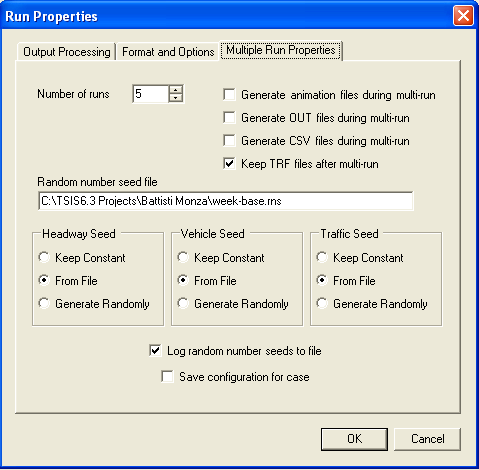
\includegraphics[width=1\linewidth]{multi-run-properties-tsis-next}\captionof{figure}[Esecuzione multipla guidata da file \acs{RNS}]{Selezione del file \acs{RNS} per l'impostazione dell'esecuzione multipla.}\label{fig:multi-run-properties-tsis-next}
	\end{minipage}
	\item si esegua la simulazione cliccando sull'apposito pulsante
	\item conclusa la simulazione, \acsfont{Sensors} \acs{DLL} salva, nella cartella dove il file \acs{TRF} simulato risiede, i file \acs{CSV} di output (riguardo il cui formato si è discusso nella \autoref{subsec:sensors-dll-output}~\vpageref{subsec:sensors-dll-output}).
\end{itemize}

Si osservi che per ogni esecuzione della simulazione viene generato il relativo file di output. Il nome di tali file \acs{CSV} è una concatenazione delle seguenti informazioni: nome del file \acs{TRF} (seguito dal numero dell'esecuzione in caso di esecuzione multipla), data e ora dell'esecuzione, suffisso \lstinline[]|sensors|.

\subsection{Applicativi di supporto}
Ottenuti i file di output di \acsfont{Sensors} \acs{DLL} è necessario trasformarli in un dataset utile al framework delle \acs{CTBN}. A tale scopo sono stati sviluppati degli applicativi, brevemente discussi nella \vref{sec:dataset-tools}.

Il primo passo necessario consiste nella sostituzione dei \emph{\keyword{time period}} con le rispettive classi (si veda a tal riguardo la \vref{tab:ds-2-tp-labels}). A tale scopo è stato sviluppato un programma in linguaggio \lstinline[]|R| con interfaccia \lstinline[]|bash| chiamato \lstinline[]|sensors2dataset|.

Riguardo al modello in questione è quindi necessario eseguire il succitato programma nel seguente modo, ripetendo tale passo per tutti i $5$ file di output generati (si ricorda che il modello per i giorni lavorativi viene eseguito infatti $5$ volte, una per ogni giorno lavorativo):

\vspace*{8pt}\inputsourcecode[caption={[Sostituzione dei \emph{time period} con le relative classi]Esecuzione del programma \lstinline[]|bash| per la sostituzione dei \emph{\keyword{time period}} con le relative classi nel file \acs{CSV} relativo al \ds{2}.},language=sh,basicstyle=\footnotesize\ttfamily,numbers=none,label=lst:sensors2dataset]{codes/sensors2dataset2}
Di seguito si spiegano brevemente le opzioni utilizzate:
\begin{itemize}
	\item l'opzione \lstinline[]|i| serve a specificare il percorso del file di input, cioè del file \acs{CSV} generato da \acsfont{Sensors} \acs{DLL}
	\item l'opzione \lstinline[]|t| comunica al programma che il file di input è dotato di intestazione
	\item l'opzione \lstinline[]|r| comunica al programma di rimuovere la colonna relativa ai \emph{\keyword{time period}}
	\item l'opzione \lstinline[]|b| serve a definire i \emph{\keyword{time period}} a partire dai quali una nuova classe deve essere creata e associata
	\item l'opzione \lstinline[]|v| serve per eseguire il programma in modo verboso.
\end{itemize}
Si osservi tuttavia che \lstinline[]|sensors2dataset| implementa molte altre opzioni la cui descrizione è stata tuttavia tralasciata.

Infine, si noti che \lstinline[]|sensors2dataset| non sovrascrive il file di input. Infatti, esso genera automaticamente un nuovo file con le modifiche apportate, concatenando al nome del file di input il suffisso \lstinline[]|dataset|.

A questo punto è possibile scegliere una granularità temporale qualsiasi con cui tagliare il file \acs{CSV}, tenendo presente che \acsfont{Sensors} \acs{DLL} utilizza per il monitoraggio del passaggio dei veicoli sui sensori la massima granularità temporale ottenibile da \acs{CORSIM}, cioè $0.1$ secondi.

Di conseguenza, ipotizzando di voler tagliare il corrente file \acs{CSV} in più file da $100$ secondi, si utilizza il programma \lstinline[]|bash| appositamente sviluppato a tale fine, \lstinline[]|splitfile|.
\vspace*{8pt}\inputsourcecode[caption={[Generazione del \ds{2}]Esecuzione del programma \lstinline[]|bash| finalizzato alla generazione del \ds{2}. Il file di input viene tagliato in più file, ognuno dei quali rappresentante un intervallo temporale di $100$ secondi.},language=sh,numbers=none,basicstyle=\small\ttfamily]{codes/splitfile2}
L'opzione \lstinline[]|n| serve a specificare il numero di righe da cui ogni file deve essere composto. In questo caso quindi, poiché ogni riga rappresenta un intervallo temporale di $0.1$ secondi e desideriamo ottenere dei file che rappresentino intervalli temporali minori o uguali di $100$ secondi, impostiamo il suo valore pari a $1000$.

Si osservi che \lstinline[]|splitfile| salva i file generati in una nuova cartella la cui posizione corrisponde a quella del file di input.

Infine, è possibile ottimizzare il dataset appena generato rimuovendo le righe che corrispondono a intervalli temporali durante i quali non è avvenuta alcuna transizione di stato per nessun sensore. A tale scopo viene fornito un programma \lstinline[]|bash| chiamato \lstinline[]|killconsdup|. Esso permette l'ottimizzazione di un singole file \acs{CSV} secondo la logica descritta oppure l'ottimizzazione di tutti i file \acs{CSV} presenti nella cartella di input fornita. Di seguito si illustra la seconda tipologia d'utilizzo di \lstinline[]|killconsdup|.
\vspace*{8pt}\inputsourcecode[caption={[Ottimizzazione del \ds{2}]Esecuzione del programma \lstinline[]|bash| finalizzato alla rimozione delle osservazioni duplicate, cioè delle righe relative agli intervalli temporali durante i quali tutti i sensori sono rimasti nel loro precedente stato.},language=sh,numbers=none]{codes/killconsdup2}
Si osservi che \lstinline$killconsdup$ non considera la prima riga dei file che processa, assumendo che essa contenga l'intestazione del file \acs{CSV}. Inoltre esso non considera la prima e la seconda colonna dei file di input assumendo esse si riferiscano rispettivamente alla colonna del tempo e della classe. Infine, affinché tale programma funzioni correttamente è necessario che il separatore dei file \acs{CSV} di input sia la virgola.

Eseguito il precedente comando, i file che compongono il dataset saranno sovrascritti con la loro rispettiva versione ottimizzata.
